\documentclass{article}

% ready for submission
\usepackage[final]{neurips_2021}
\usepackage[utf8]{inputenc} % allow utf-8 input
\usepackage[T1]{fontenc}    % use 8-bit T1 fonts
\usepackage{hyperref}       % hyperlinks
\usepackage{url}            % simple URL typesetting
\usepackage{booktabs}       % professional-quality tables
\usepackage{amsfonts}       % blackboard math symbols
\usepackage{nicefrac}       % compact symbols for 1/2, etc.
\usepackage{microtype}      % microtypography
\usepackage{xcolor}         % colors
\usepackage{enumitem}
\usepackage{fancyhdr}
% \usepackage{algorithmicx, algpseudocode, algorithm, float}
\usepackage{algorithmicx, algorithm, float}
\usepackage[noend]{algpseudocode}
\usepackage{graphicx}
\graphicspath{ {images/} }
\usepackage{wrapfig}
\usepackage{subfigure}
\usepackage{caption}
\usepackage{subcaption}

%\usepackage[T1]{fontenc}    % use 8-bit T1 fonts
%\usepackage{hyperref}       % hyperlinks
%\usepackage{url}            % simple URL typesetting
%\usepackage{booktabs}       % professional-quality tables
%\usepackage{amsfonts}       % blackboard math symbols
%\usepackage{nicefrac}       % compact symbols for 1/2, etc.
%\usepackage{microtype}      % microtypography
%\usepackage[dvipsnames]{xcolor}        % colors

%\usepackage[utf8]{inputenc}
%\usepackage{multicol,multirow}
%\usepackage{amsmath}
%\usepackage[legalpaper, margin=1in]{geometry}

\title{CS271 Project Final Draft: Sokoban}

\author{
  Nitya Raju\\
  Department of Computer Science\\
  University of California, Irvine\\
  Irvine, CA 92697\\
  \texttt{nraju1@uci.edu} 
   \And
  Akshita Singh \\
  Department of Computer Science\\
  University of California, Irvine\\
  Irvine, CA 92697\\
  \texttt{akshis2@uci.edu} 
   \And
  Almendra Salgado Gatica \\
  Department of Computer Science\\
  University of California, Irvine\\
  Irvine, CA 92697\\
  \texttt{arsalgad@uci.edu} 
}
\begin{document}

\maketitle

%\begin{abstract}

%  The abstract paragraph should be indented \nicefrac{1}{2}~inch (3~picas) on
%  both the left- and right-hand margins. Use 10~point type, with a vertical
%  spacing (leading) of 11~points.  The word \textbf{Abstract} must be centered,
%  bold, and in point size 12. Two line spaces precede the abstract. The abstract
%  must be limited to one paragraph.
%\end{abstract}

\section{Abstract}
Sokoban is a challenging puzzle for both humans and AIs. Researchers have invested in implementing and improving multiple Reinforcement Learning algorithms - ranging from Monte Carlo Tree Search to Q-Learning - to make Sokoban reach goals faster as the boards get more complex. In our paper, we implement a Q-Learning algorithm that goes beyond the conventional decision of inheriting the entire board as the state space, and instead explores the possibility of reducing it just the exact box locations. We then re-define our Q-value update approach to be driven by the box locations as against the entire Sokoban environment. The reduced branching factor and run-time are an acceptable trade-off to the more convoluted state structure. When compared to other Q-Learning variations, such as Deep Q-Learning, that we also tried, this emphasis on re-examining our reinforcement learning environment itself rendered much better results with respect to game success and efficiency. 

\section{Introduction}

Sokoban is a part puzzle, part video game in which a player (Sokoban) pushes around boxes such that they end up in storage locations which are pre-determined by a game level. Sokoban runs into walls and other boxes along the way and whether or not it can navigate its way around such roadblocks is what forms the crux of this game. 

We have developed an AI agent for Sokoban. Our project aims to develop a reasonably intelligent AI Sokoban that can handle multiple configurations of walls, boxes, and storages, all with varying complexities. We called on to the Q-Learning algorithm from within the larger umbrella of Reinforcement Learning and Markov Decision Processes to perform this taks (see \textbf{Q-Learning Algorithm}. Besides that, we invested in identifying some efficient approaches to identifying as many deadlock scenarios as possible, if not all (see \textbf{Freeze Deadlock Detection}). And finally, we constructed some macro moves the re-defined the state space to be limited to the box locations, thereby reducing our state space and branching factor exponentially (see \textbf{Macro Moves}). 

% \section{Reinforcement Learning and Q- Learning}
% \textbf{What is Reinforcement Learning?}: \\
% Reinforcement Learning (RL) essentially entails decision making in an unknown and stochastic environment. To support this decision making, we call on to some of the following elements of RL: \emph{Rewards, Value Functions, Policies}. For Sokoban, this Rewards would look something like this: 

% a) (+100) for a move that leads to a ("win"

% b) (-100) for a move that creates a deadlock

% c) (-10) for a move that kicks a box out of a storage location

% d) (+10) for a move that pushes a box into a storage location

% e) (+5) for a move that pushes a box without creating a deadlock**

% f) (-1) for a move into empty square that does not create a deadlock***
% \\
% * Win: the move that pushes the last remaining box not in a storage location into a storage location \\
% ** Deadlock: a deadlock that we have been able to capture \\
% *** We do penalize a move with a negative score even if its in the right direction, because our goal is to push the boxes into storage locations as quickly as possible. \\
% \\
% RL algorithms can be broken down based on whether they are model-dependent or model-free. For Markov Decision Processes (MDP) the "model" largely consists of state transition probabilities and rewards: $<S, A, P, R, \gamma>$. Temporal Difference Leaning (TD) is the subset of RL algorithms that do not have these transition probabilities and rewards explicitly defined. Learning happens through "episodes of experience". The two common algorithms within TD are Q-Learning and SARSA. 
% \\
% \\
% \textbf{What is Q-Learning?}:
% Q-Learning is a TD algorithm that learns action values relative to the greedy policy. A Q-Learning algorithm follows the greedy policy with with some probability < epsilon, and the optimal policy with the probability (1 - epsilon). This is in contrast to SARSA, which learns action values relative to the policy it follows. \\
% % SARSA: $Q(S,A) \leftarrow Q(S,A) + \alpha(R + \gamma Q(S',A') - Q(S,A))$ \\
% Q-Learning: $Q(S,A) \leftarrow Q(S,A) + \alpha(R + \gamma max_{\alpha'}Q(S',A') - Q(S,A))$  \\
% where: \\
% $S$ is the current state  \\
% $A$ is the current action \\
% $S'$ is the next state \\
% $A'$ is the next action \\
% $R$ is the reward \\
% $\alpha$ is the discount rate \\
% $\gamma$ is the learning rate \\
% $Q(S,A)$ is the Action Function at the current state $S$ with current action $A$ \\
% $Q(S',A')$ is the Action Function at the next state $S'$ with next action $A'$ \\
% \\
% \\
% \textbf{Why Q-Learning}
% Sokoban is a puzzle with very few consistencies to exploit. Our AI Sokoban has no idea where the walls, boxes, and storage locations would be as we take it from one level to another. The real "reward" is successfully pushing all boxes in storage locations. Thus Sokoban is a game with sparse rewards and not much information and consistencies to with. This makes it apt for an algorithm that learns and improves along the way, instead of waiting for the whole episode to get over to learn anything at all. \\ \\
% At each step, Q Learning computes the error after learning from a policy outside its domain $\alpha(R + \gamma max_{\alpha'}Q(S',A') - Q(S,A))$ and updates $Q(S,A)$ accordingly. Because Q-Learning does not follow an policy, it can continue learning while changing policies. This flexibility of changing policies and hence ensuring optimality is what drew us towards Q-Learning as against SARSA. 

\section{Approach To Game Development}

We modularised our program and broke it down into 3 modules: 1) Agent, 2) State, and 3) Game.

\algdef{SE}% flags used internally to indicate we're defining a new block statement
[STRUCT]% new block type, not to be confused with loops or if-statements
{Struct}% "\Struct{name}" will indicate the start of the struct declaration
{EndStruct}% "\EndStruct" ends the block indent
[1]% There is one argument, which is the name of the data structure
{\textbf{struct} \textsc{#1}}% typesetting of the start of a struct
{\textbf{end struct}}% typesetting the end of the struct

\subsection{Agent}
The Agent class focused on the actions Sokoban would take given the rules of the game and the constraints of Q Learning Algorithm. 

\begin{algorithm}
\floatname{algorithm}{Class}
\caption{Agent}
\begin{algorithmic}
\Struct{Agent(object)}
  \State $row$ : Actual row position in the board
  \State $col$ : Actual column position in the board
  \State $state$ : State object
  \State $epsilon$ : Fraction of the time agents acts randomly
  \State $gamma$ : Discount factor
  \State $learning$ : Also known as alpha
  \State $actions$ : Basic actions: LEFT, RIGHT, UP, DOWN
  \State $history$ : Record of state and action taken from that state
  \State $q$ : Q values \\
  \State $paths$ : visited paths \\

  \State def $agentMove(self, state)$
  \State def $movePlayer(self, data, state, action)$
  \State def $qValueUpdate(self, update)$
  \State def $possiblemoves(self, state, box locations)$
  \State def $reachablesBoxes(self, board, agent location, goal)$
  
\EndStruct
\end{algorithmic}
\label{Class}
\end{algorithm}

We described 3 principal methods in this class:
    
\begin{enumerate}[label=\alph*)]
    \item \underline{AgentMove}: This function returns the action Sokoban takes using an $\epsilon$-greedy policy. This means Sokoban takes a random action with probability $\epsilon$ (initialized to $0.1$) and acts according to the policy it learns the remaining time. The pseudo-code for the same is described in detail in the next section.
    \item \underline{MovePlayer}: This function implement Sokoban's move given the rules of the game. It looks into the surrounding region once the agent takes an action and informs the game of any boxes Sokoban moved, or any obstacles (walls, deadlocks, bounds) that it confronted along the way. 
    \item \underline{qValueUpate}: This function updates the current q-value by loyally following the Q-Learning algorithm formula. The pseudo-code for this function is also detailed out in the next section. 
    \item \underline{reachableBoxes and possibleMoves}: These two functions our part of macro moves focus, wherein we redefine the state space to be limited to boxes and also redefine q-values as dictionaries of dictionaries guided by possible actions given a box location. The pseudo code of these algorithms are in the section Macro Moves. 
\end{enumerate}

\subsection{State}
The state class plays the important role of deciding the fate of Sokoban given the level it has been placed into. It takes the level parameters (coordinates of the agent, walls, boxes, and goals) to construct the initial board. And with that information, Sokoban decides how to go about getting to the goal as quickly possible, with the help of the Agent class. 

\begin{algorithm}
\floatname{algorithm}{Class}
\caption{State}
\begin{algorithmic}
\Struct{State(object)}
  \State $rows$ : Number of rows in the board
  \State $cols$ : Number of colums in the board
  \State $numWalls$ : Number of walls
  \State $walls$ : Walls location in the board
  \State $numBoxes$ : Number of boxes
  \State $boxes$ : Boxes location in the board
  \State $numStorage$ : Number of storages
  \State $storage$ : Storage location in the board
  \State $playerCol$ : Player inital column location 
  \State $playerRow$ : Player inital row location
  \State $board$ : Board creation for graphics
  \State $safeSquares$ : Position of safe squares to move a box
  \State $simpleDeadlocks()$ \\
  
  \State def $createBoard(self)$
  \State def $simpleDeadlocks(self)$
  \State def $depthFirstSearch(self, boxLocation)$
  \State def $checkBoard(self, data, action)$
  \State def $isGameOver(self, data, update)$
  \State def $isDeadlock(self, pos, obs))$
  \State def $freezeDeadlockDetection(self, state, box positions, blocked positions, previously evaluated positions, axes))$
\EndStruct
\end{algorithmic}
\label{Class}
\end{algorithm}

We described 3 principal methods in this class:
    
\begin{enumerate}[label=\alph*)]
    \item \underline{createBoard}: This function creates the structure of the board as specified by the project spec. 
    \begin{figure}[htp]
        \centering
        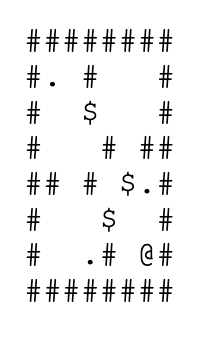
\includegraphics[width=2cm]{Input.png}
        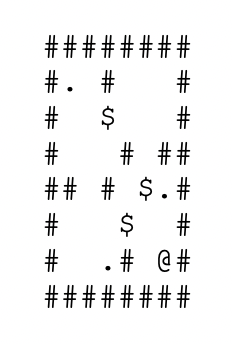
\includegraphics[width=4cm]{board.png}
        \caption{\emph{createBoard} takes in the input string and creates the Sokoban board}
    \end{figure} 
% perhaps show a picture of a board with all the ###, $$$, @, ..
    \item \underline{checkBoard}: Given an action that takes Sokoban to an existing box location, this function returns the possible situations that the box might end up in if pushed. There are 4 such possible situations:
    
    \begin{enumerate}[label=\arabic*)]
        \item The box moves onto a storage location. 
        \item The box moves off of a storage location (this happens in case Sokoban ends up on a storage location).
        \item The box takes on the position next to a wall or another box in which case we might be in a deadlock position.
        \item The box moves into an empty square. 
    \end{enumerate}
    
    \item \underline{isDeadlock} and \underline{SimpleDeadlock}: These functions implement 2 common deadlock scenarios, the details and pseudo-codes of which are discussed at length in the Deadlock Detection section. 
\end{enumerate}

\subsection{Game}

This module essentially implements the Sokoban game. It consists of an assortment of functions that ensures Sokoban's timely movements. An important function is this module is \underline{timerFired}, which keeps the game going while its not over. In particular, it keeps calling on the following functions as long as we have not hit any of the criteria which end the game: 


\begin{enumerate}[label=\alph*)]
    \item \underline{agentMove}: ensures Sokoban keeps taking Q-Learning informed action.
    \item \underline{qValueUpdate}: ensures the q-values keep getting getting updated according the Q-Learning formula. 
    \item \underline{movePlayer}: keeps moving Sokoban as long as the win condition has not been met, a deadlock has not been detected and we have not timed out.
    \item \underline{checkBoard}: keeps updating on a the results of the action taken by the agent, which could be moving a box, winning the game or reaching a deadlocked position.
\end{enumerate}

\begin{algorithm}
    \caption{\textsc{timerFired}: Play the game}\label{euclid}
    \hspace*{\algorithmicindent} \textbf{Input}: struct that groups an agent and state \\
    \begin{algorithmic}
    \If{isNotGameOver} 
        \State $agent.agentMove$ Get action from $\epsilon$-greedy policy
        \State $state.checkBoard$ Check for outcome
        \State $agent.movePlayer$ Move the player through the board
        \State $agent.qValueUpdate$ Update Q values
    \EndIf 
    \end{algorithmic}
\end{algorithm}

{
\begin{wrapfigure}{l}{0.19\textwidth} %this figure will be at the right
    \centering
    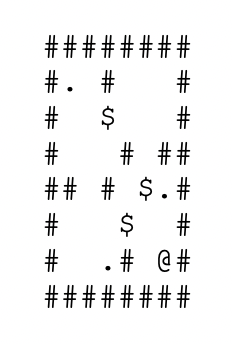
\includegraphics[width=0.19\textwidth]{board.png}
\end{wrapfigure}

As a very basic graphic design, we use Canvas\footnote{https://tkdocs.com/tutorial/canvas.html} to implement a rudimentary Sokoban GUI game. 

\begin{enumerate}[label=\alph*)]
    \item Player: It is represented as an \textbf{Red Circle}.
    \item Box: It is represented as an \textbf{Brown Rectangle}.
    \item Wall: It is represented as an \textbf{Beige Rectangle}.
    \item Storage: It is represented as an \textbf{Pink Circle}.
\end{enumerate}
}

\section{Q-Learning Algorithm}

\paragraph{Why Q-Learning}
Sokoban is a puzzle with very few consistencies to exploit. Our AI Sokoban has no idea where the walls, boxes, and storage locations would be as we take it from one level to another. The real "reward" is successfully pushing all boxes in storage locations. Thus Sokoban is a game with sparse rewards and not much information and consistencies to with. This makes it apt for an algorithm that learns and improves along the way, instead of waiting for the whole episode to get over to learn anything at all.

At each step, Q-Learning computes the error after learning from a policy outside its domain $$\alpha(R + \gamma max_{\alpha'}Q(S',A') - Q(S,A))$$ 
and updates $Q(S,A)$ accordingly. Q-Learning allows the agent to continue learning while changing updating the policies. This flexibility of changing policies and hence ensuring optimality is what drew us towards Q-Learning as against SARSA. 

We set discount factor $\gamma$ to $0.9$ as we want to agent to value long term rewards as too much short sightedness can lead to early game deadlocks. The agent chooses moves according to an $\epsilon$-greedy policy, where $\epsilon$ is initially $0.1$. We want to find a balance between exploration and exploitation where the agent spends spends some time exploring new moves and the remaining time acting according according to learned policy. We initialize the learning rate $\alpha$ to $0.5$. We can reduce the values of $\alpha$ and $\epsilon$ as the agent learns so we eventually converge to an optimal policy. 

The agent selects moves according to an $\epsilon$-greedy policy. With probability $\epsilon$, the agent moves in one of the cardinal directions randomly. The remaining time, the agent chooses a move given it's current state that has the maximum q value. This allows us to find the right balance between exploring new moves and exploiting existing knowledge.  $\epsilon$ is initially chosen to be $0.1$ and this value is decreased over time so the behaviour of the agent eventually converges. Discount factor $\gamma$ is set to $0.9$ so the agent will value long term rewards. The learning rate $\alpha$ is set to $0.5$.

\begin{algorithm}
    \caption{\textsc{agentMove}: Function that decides Agent Move based on Q-Learning Algorithm}\label{euclid}
    \hspace*{\algorithmicindent} \textbf{Input}: \emph{state} of the board \\
    \hspace*{\algorithmicindent} \textbf{Output}: \emph{action} according to the Q-Learning  Algorithm \\
    \begin{algorithmic}
    \State $state \gets$ the structure of the board as defined by walls, boxes etc.
    \State $actions \gets$ a list of possible moves (up, down, left right)
    \State $q \gets$ a dictionary that maps the state to q values possible for that state
    \State $epsilon \gets$ Initialize to some number between 0 and 1
    \State $probability \gets$ Randomly select between 0 and 1 \\
    \If{$ probability < epsilon$} 
        \State Randomly select a move
    \Else
        \If {If current state matches the state (key) within the action function (q)}  % need to revisit explanation
            \State $qScore \gets$ the q values for the 4 actions that correspond to the current state
            \State $action \gets$ take the action that corresponds to the action with highest $qScore$
        \Else
            \State Initialize current state in the dictionary, with q values for all possible actions initialized to 0
            \State Select a random action from the 4 possible actions
        \EndIf
    \EndIf 
    \end{algorithmic}
\end{algorithm}

\begin{algorithm}
    \caption{\textsc{qValueUpdate}: Function to Update Q Values Using the Q-Learning Formula}\label{euclid}
    \hspace*{\algorithmicindent} \textbf{Input}: result of an action \emph{update} (ex. deadlock, goal etc. \\
    \hspace*{\algorithmicindent} \textbf{Output}: None (the function updates Q Value) \\
    \begin{algorithmic}
    \State $update \gets$ record of what does an action result in (ex: deadlock, goal etc.) 
    \State $history \gets$ history of all \emph{states} and \emph{actions} up until the last one
    \State $reward \gets$ reward on taking a certain action, initially set to -1
    \State $\alpha \gets$ Discount rate, which is some constant between 0 and 1
    \State $\gamma \gets$ Learning rate, which is Some constant between 0 and 1
    %// Get second last (time t) and last (time) actions and states from the history 
    \State $s_0 \gets$ second last state (at time $t$)
    \State $s_1 \gets$ last state (at time $t+1$)
    \State $a_0 \gets$ second last action (at time $t$)
    \State $a_1 \gets$ last action (at time $t+1$) \\
    
    \If{action results in a deadlock}
        \State $reward = -100$
    \ElsIf{action results in all boxes in storage location}
        \State $reward = 100$
    \ElsIf{action results in some box in a storage location}
        \State $reward = 10$
    \ElsIf{action results in all boxes being pushed out of a storage location}
        \State $reward = -10$
    \ElsIf{action results in a box not on a storage location to a square also not a storage location}
        \State $reward = 5$
    \ElsIf{action results in the agent moving without impacting the box in anyway}
        \State $reward = -1$
    \EndIf \\
    
    \State $currQValue \gets$ the current Q value
    %// Update the q-value using the formula $Q(S,A) \leftarrow Q(S,A) + \alpha(R + \gamma max_{\alpha'}Q(S',A') - Q(S,A))$ \\
    \State $q[s_0][a_1] \gets q[s_0][a_0] + \alpha * (reward + \gamma * (max(q[s_1][a_1]) - currQValue))$
    \end{algorithmic}
\end{algorithm}

\section{Deadlock Detection}

Sokoban is the kind of puzzle where many mistakes are irreversible and lead to deadlocked positions. This problem is particularly concerning if we work with RL (as compared to a search algorithm such as A*), which does not think ahead. Thus, it is imperative that we try to identify and fix as many deadlocks as possible, before the start of the game or while we are playing and before the next action is taken.  

\subsection{Types of Deadlocks}
\begin{enumerate}
    \item Corner Deadlock: box in any corner of the walls.
    \item Horizon Deadlock: box next to wall, and 
    \begin{enumerate}[label=\alph*)]
        \item There is no goal state in any possible corner where the horizon can go, or
        \item There is a goal in some corner but is blocked by a wall/another box.
    \end{enumerate}
    \item Square Deadlock: boxes all together and none of them can be moved.
    \item Dead square deadlock: just 1 push to a box to one square which creates deadlock (corner, horizon).
    \item Freeze Deadlock: pushing a box such that either it, or some other box becomes completely immovable.
    \item Corral Deadlock: area not reachable by the agent without creating a deadlock - hence the current situation is itself a deadlock
\end{enumerate}

We have tried to address some of the deadlocks in our game and plan to include others if time permits. 

\subsection{Simple Deadlock Detection Algorithm}
This function essentially flips the Sokoban game over. We start by placing the box on each possible storage location, and then we pull that box back to every possible legal square. All the squares that the box visits, starting from each possible storage location is marked as a safe location.

\begin{figure}[htp]
        \centering
        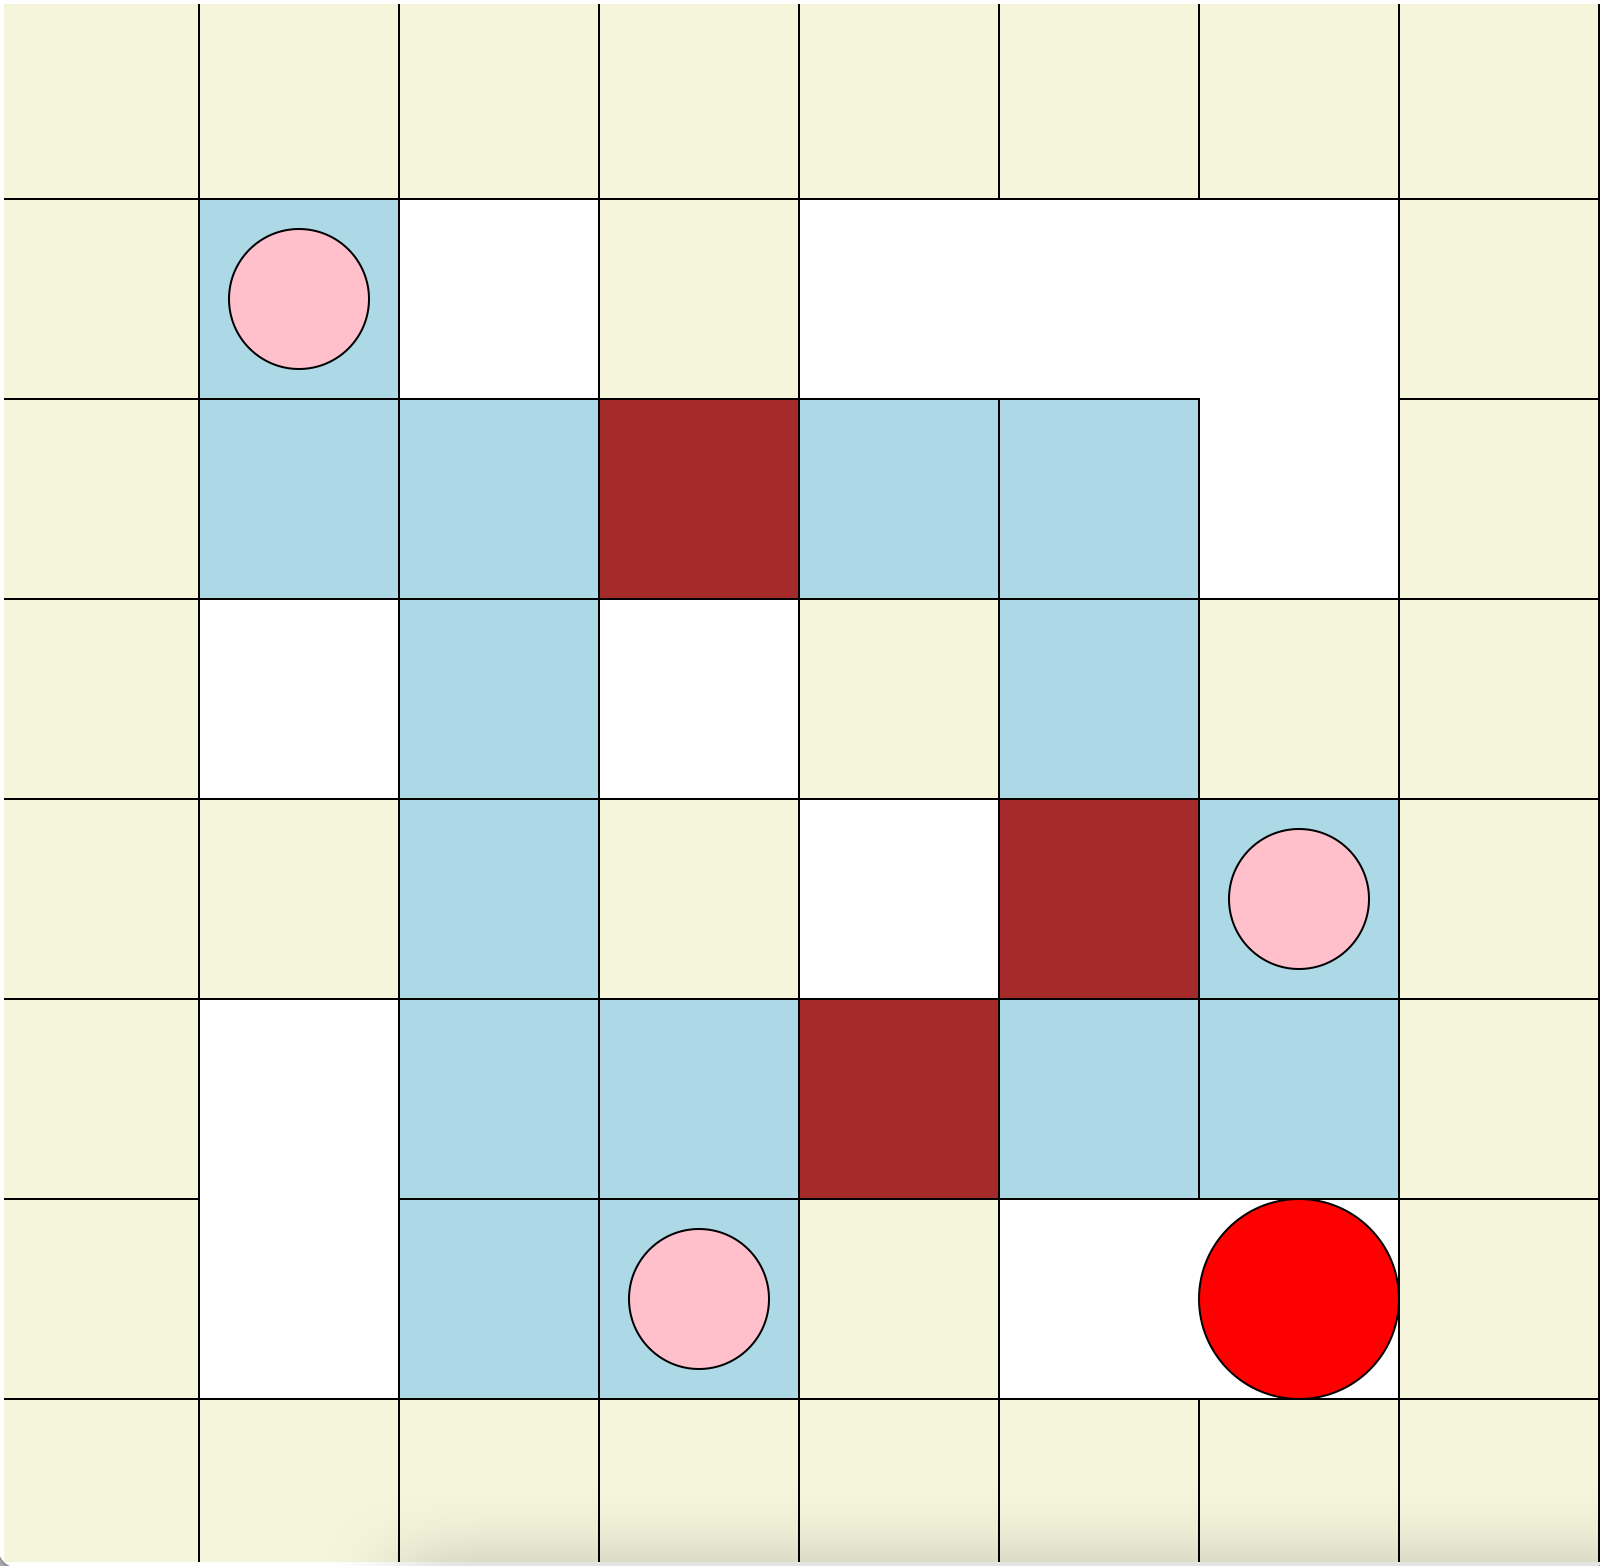
\includegraphics[width=4cm]{Deadlock.png}
        \caption{Blue squares indicate safe locations for boxes, white squares indicate simple deadlock positions that will end the game}
    \end{figure} 

\begin{algorithm}
    \caption{\textsc{simpleDeadlocks}: Simple Deadlock Detection}\label{euclid}
    \hspace*{\algorithmicindent} \textbf{Input}: location of the box \emph{boxLocation} \\
    \hspace*{\algorithmicindent} \textbf{Output}: recursive call to the Simple Deadlock Function \\
    \begin{algorithmic}
    \State $safeSquares \gets$ a square that does not create an obvious deadlock, initially an empty set
    \State $row, col \gets$ coordinates of the box location \\
    \If{the location of the box is a safe location} 
        \State do nothing
    \EndIf 
    \For{an action in \emph{action} (up, down , left, right)}
        \State $newLocation \gets$ coordinates of the box after taking an action 
        \State $twoStepsLocation \gets$ coordinates of the box after taking the same action twice \\
        \If{\emph{newLocation} within the bounds of the game level \textbf{and} \emph{newLocation} is not a wall \textbf{and} \emph{twoStepsLocation} is not a wall either}
            \State Add \emph{boxLocation} in the list of \emph{safeSquares} % need to figure out how to indent
            \State Call the Simple Deadlock Function with \emph{newLocation} as \underline{input}
        \EndIf
    \EndFor
    \end{algorithmic}
\end{algorithm}
% \newpage
%\textbf{if}
%1) \emph{newLocation} within the bounds of the game level, AND
%2) \emph{newLocation} is not a wall, AND 
%3) \emph{twoStepsLocation} is not a wall either
\newpage
\subsection{Freeze Deadlock Detection Algorithm}

This function detects if there are obstacles around the box that do not allow it to move, either walls or another boxes.

% \begin{algorithm}
%     \caption{\textsc{isDeadlock}: Freeze Deadlock Detection}\label{euclid}
%     \hspace*{\algorithmicindent} \textbf{Input}: expected position of the agent \emph{posA} \\
%     \hspace*{\algorithmicindent} \textbf{Output}: expected position of the obstacle \emph{posO} \\
%     \begin{algorithmic}
%     \State $posA \gets$ expected position of the agent
%     \State $posO \gets$ expected position of the obstacle \\
%     \If{the expected position of obstacle is above \textbf{or} below the expected position of the agent (Vertical Analysis)} 
%         \If{the square on the left the agent contain either boxes \textbf{or} walls}
%             \State return True
%         \ElsIf{the square on the right the agent contain either boxes \textbf{or} walls}
%             \State return True
%         \Else
%             \State return False
%         \EndIf

%     \ElsIf {the expected position of obstacle is to the left or right of the expected position of the agent (Horizontal Analysis)}
%         \If{the square immediately above the agent contains either boxes \textbf{or} walls}
%             \State return True
%         \ElsIf{the square immediately below the agent contains either boxes \textbf{or} walls}
%             \State return True
%         \Else
%             \State return False
%         \EndIf
%     \EndIf 
%     \end{algorithmic}
% \end{algorithm}

\begin{algorithm}
    \caption{\textsc{freezeDeadlockCheck}: Freeze Deadlock Detection}\label{euclid}
    \hspace*{\algorithmicindent} \textbf{Input}: state, box location, blocked positions, positions checked already, axes \emph{posA} \\
    \hspace*{\algorithmicindent} \textbf{Output}: boolean indicating if its a freeze deadlock scenario \\
    \begin{algorithmic}
    \If {box not in \emph{boxes}}
        \State return False
    \EndIf
    % \State $boxX, boxY \gets$ box coordinates
    \State $directions \gets$ dictionary of vertical and horizontal direction coordinates
    % \If {box is not \emph{blocked}}
    %     \State $blocked[box] \gets$ { "horizontal": False, "vertical": False}
    % \EndIf
    
    % \If {box is not \emph{blocked}}
    %     \State $checked[box] \gets$ { "horizontal": False, "vertical": False}
    % \EndIf
    
    % \If {axes is not empty}
    %     \State $axes \gets$ ["horizontal", "vertical"]
    % \EndIf
    
    % \If {axis is in ["horizontal", "vertical"]}
    %     \If {axis not in axes}
    %         \State delete blocked[box][axis]
    %     \EndIf
    % \EndIf
    
    \State $axes \gets$ horizontal and vertical axis
    
    \For {axis in axes} 
        \If {axis already checked} 
            \State $continue$
        \EndIf
        
        \State $dir1, dir2, dir3, dir4 \gets$ all axis directions
        \State $side1X, side1Y \gets$ box coordinates if pushed left/up in the horizontal/vertical axis
        \State $side2X, side2Y \gets$ box coordinates if pushed right/down in the horizontal/vertical axis
        
        \If {(side1X, side1Y) or (side2X, side2Y) either in \emph{walls} or not in \emph{safeSquares}}
            \State blocked[box][axis] = True (mark box axis as blocked )
        \EndIf
        
        \State  $checked[box][axis] \gets$ true (mark box axis as checked) 
        \State (recursively check for blocked boxes on either side that are not already checked)
        
        % (Check if thhe next box is blocked, and if so check recursively all the way through)
        \If {(side1X, side1Y) in \emph{boxes}}
            \If{\emph{freezeDeadlockCheck}(data, (side1X, side1Y), blocked, checked, [otherAxis(axis)])}
                blocked[box][axis] = True (mark box axis as blocked )
            \ElsIf {\emph{checked}[(side1X, side1Y)][axis] is True}
                \If {\emph{blocked}[(side1X, side1Y)][axis] is True}
                    \State blocked[box][axis] = True
                \EndIf
            \EndIf
        \EndIf
        \State (repeat the  the above section for the other side (side2X, side2Y)
    \EndFor
        
    % \If {axes is empty} (base case)
    %     \For {box in blocked}
    %         \For {axis in blocked[box]}
    %             \If blocked[box][axis] is False (axis for that box is not blocked)
    %                  \State return False
    %             \EndIf
    %         \EndFor
    %     \EndFor
        
    % \Else % (recursive case)
    %     \For {axis in blocked[boxes}
    %         \If {blocked[box][axis] is False (axis for the box is not blocked)}
    %             \State return False
    %         \EndIf
    %         \State return True
    %     \EndFor
    % \EndIf
    
    \end{algorithmic}
\end{algorithm}

\newpage

\section{Redefining State Space - Macro Moves}
The overarching goal of macro moves is to \underline{reduce the state space}, thereby making our AI learn faster and better. Considering the entire board as a state space is implementation friendly but not particularly efficient. This is because every time Sokoban makes a move, the entire state space (that is, the board) changes. In fact, even when it's considering a move, it's looking at 4 different boards. \\
With macro moves, we introduce a completely different state space, which is represented by the positions of the boxes. In this view, an action does not have to change the state space. Thus, there's a lot less information for Sokoban to digest. This new view also reduces our branching factor by a lot. \\
Changing states spaces in this fashion also changes how we handle Q-value. Up until now, we have represent q-values as list of 4 numbers, 1 for each possible. Now, we first specify the box that Sokoban wants to target, which then helps it choose an action. Thus, the q-value representation now shifts to the form of dictionary of dictionaries (for boxes, and possible actions for each box). 

\begin{algorithm}
    \caption{\textsc{possibleMoves}: Proactively Identify Legal Moves}\label{euclid}
    \hspace*{\algorithmicindent} \textbf{Input}: State, (box positions), selected box position, agent location\\
    \hspace*{\algorithmicindent} \textbf{Output}: legal moves
    \begin{algorithmic}
    % \State $legalMoves \gets$ an empty list that would store all legal moves
    % \State $row, col \gets$ coordinates of the box
    % \State $agentX, agentY \gets$ coordinates of the agent
    % \State $visited \gets$ visited paths from Sokoban to the box
    
    \For{an action in \emph{action} (up, down , left, right)}
        \State $newRow, newCol \gets $ new box coordinates after an action is taken
        % \State $boxRow, boxCol \gets $ coordinates of the box
        % \State $newBoxX, newBoxY \gets $ new box coordinates after adding action coordinates
        % \State $newAgentX, newAgentY \gets $ new agent coordinates after subtracting action coordinates
        \If {new agent coordinates not in 1) a visited path \textbf{or} 2) walls \textbf{or} 3) boxes }
            \State $continue$
        \EndIf
        % new position of the box after the action
        \If {(newRow, newCol) \textbf{not in} walls or boxes \textbf{and within} row and column dimensions}
            \State add action coordinates to list of legal moves
        \EndIf
    \EndFor
    \end{algorithmic}
\end{algorithm}

\begin{algorithm}
    \caption{\textsc{reachableBoxes}: boxes that can be reached starting ate current agent position}\label{euclid} 
    \hspace*{\algorithmicindent} \textbf{Input}: board, agent location, goal \\
    \hspace*{\algorithmicindent} \textbf{Output}: recursive call to function that finds path from agent location to goal 
    \begin{algorithmic}
    % \State $maze \gets$ board
    % \State $rows,cols \gets$ count of rows and columns in the board
    \State $visited \gets$ an empty set which will store all location reachable by Sokoban
    \State $targetRow, targetCol \gets$ goal coordinates \\
    \State \textbf{def} $solve$ (row, col)
    % try to make a move 

    \begin{algorithmic}
        \If {agent has already visited a certain path} % if you hit something you've see before then stop and don't move 
            \State return False (stops repeated evaluation of a visited path)
        \EndIf 
        \State add (row, col) to visited paths set% add it to a visited set 
        \If {(row, col) is a goal} 
            \State return True 
        \EndIf
        
        % Recursive case -
        % Take one step and see if there's a path that reaches the goal in that direction
        % If there is a such a path, return it 
        \For {an action in actions}
            \If {action leads to goal}
                
                \State (recursively call \emph{solve} to check if the path leads to goal - one step at a time)
                %if solve = true means if there is a solution in the path
                \If {\emph{solve} (row + action[0), col + action[1])}
                    \State return True
                \EndIf
            \EndIf
        \EndFor
        % no solution in this direction so remove (already checked so never going back again 
        \State remove (row, col) from visited (no path to goal in that direction so remove from consideration)
        
        % \State return False (didn't find sol'n in that path)
    \State return \emph{visited} (reachable squares from agent location) if \emph{solve}(row, col) (there is a path from the agent location to goal) else None
    
    \end{algorithmic}
    % returns reachable squares from agent's location 
    \end{algorithmic}
\end{algorithm}

\section{Results}
\subsection{Before Freeze Deadlocks and Macro Moves}
\begin{center}
\vspace{-5pt}
\footnotesize
\begin{tabular}{|c|c|c|c|c|}
    \hline
    Board & Boxes & Solution Found? & Time & Branching Factor\\
    \hline
    -01 & 4 & Yes (267) & 1/326s & --\\
    \hline
    -02 & 4 & Yes (2) & 0/187s & --\\
    \hline
    -04 & 4 & No & 354s & --\\
    \hline
    -05a & 2 & Yes (34) & 0/554s & --\\
    \hline
    02 & 10 & No & 67s & --\\
    \hline
\end{tabular}
\vspace{-5pt}
\end{center}


%\emph{posA} $\leftarrow$ expected position of the agent \\ 
%\emph{posO} $\leftarrow$ expected position of the obstacle \\

%\textbf{if} the expected position of obstacle is above or below the expected position of the agent (Vertical Analysis) \\
%(if \emph{posO[0]} $\textless$ \emph{posA[0]} or \emph{posO[0]} $\textgreater$ \emph{posA[0]})

%\textbf{if} the square on the left the agent contain either boxes or walls: return True

%(if \emph{(posA[0], posA[1] - 1)} in self.boxes or \emph{(posA[0], posA[1] - 1)} in self.walls: return True)

%\textbf{elif}  the square on the right the agent contain either boxes or walls: return True

%(elif \emph{(posA[0], pos[1]} + 1) in self.boxes or \emph{(posA[0], posA[1] + 1)} in self.walls: return True)

%\textbf{else} return False
%\textbf{elif} the expected position of obstacle is to the left or right of the expected position of the agent (Horizontal Analysis) \\
%(if \emph{posO[0]} $\textless$ \emph{posA[0]} or \emph{posO[0]} $\textgreater$ \emph{posA[0]})

%\textbf{if} the square immediately above the agent contains either boxes or walls: return True

%(if \emph{(posA[0] - 1, posA[1])} in self.boxes or \emph{(posA[0] - 1, posA[1])} in self.walls: return True)

%\textbf{if} the square immediately below the agent contains either boxes or walls: return True

%(if \emph{(posA[0] + 1, posA[1])} in self.boxes or \emph{(posA[0] + 1, posA[1])} in self.walls: return True)

%\textbf{else} return False
\newpage

\section{Future Considerations}
The Sokoban AI can be improved further with some the following considerations:
\begin{enumerate}
    \item More deadlock detections: Thus far, we have accounted for Simple deadlocks (using pullback DFS strategy), and Freeze deadlocks (using the vertical/horizontal neighborhood search strategy). We can make the agent smarter by identifying more deadlock patterns. In particular, Corral deadlock algorithms would contribute to the game's efficiency.
    % \item Macro Moves: Currently our model uses movement in the cardinal directions as actions the agent can take. By defining the actions the agent can take to be macro moves (for example a move could be, move to the nearest box not on a storage location and move it in one of the four directions). This would reduce a lot of time spent in exploration as currently the agent spends a lot of time moving in the board without interacting with any boxes.
    \item Heuristics: The agent moves according to an $\epsilon$-greedy policy so it either moves randomly or according to the policy learned so far. We can use heuristics such as distance to a box and expected number of moves to move a box to a goal to improve the performance of the agent, especially in the early game when most q values are still $0$. 
    \item Deep Q-Learning: As our state (and action) space gets larger as the levels get more complicated, a tabular record of the states and actions can become more and more cumbersome and inefficient. In such scenarios, calling on to deep neural networks to help us generalize across states.
    % \item Macro moves: Currently our implementations gives the agent four possible moves from every location on the board - Up, Down, Left, Right. We can reduce the time the agent spends exploring the board by grouping simple moves into macro moves - for example by defining one move to be move to the nearest box and push it one step. 
    % \item Heuristics: We can further inform our agents decisions by using heuristics to guide it's behaviour. For example, we could use distance to boxes that are not on storage locations, expected number of moves to move a box to a storage location to reduce the time the agent spends moving without interacting with any boxes. 
    \item Identifying special cases: Although including a special instance can be very risky in case it fails on higher levels, if we can confidently deduce some universal scenarios and account for them then that might make our algorithm a lot smarter. Nonetheless, we have chosen to not include any such cases as of now so as to push most of our improvements through Q-Learning. 
    \item Further redefine state space: We can consider including agent locations to the state space along with the box locations as well (state space = number of boxes + 1). Additionally, we can look into other state space representations as well (which aren't the whole board)   
\end{enumerate}

%\section{Random - DELETE LATER}
%https://www.researchgate.net/post/Reinforcement-learning-vs-heuristic-search \\
%https://github.com/XUHUAKing/sokoban-qlearning/blob/master/sokoban-solver-final-report.pdf \\
%https://github.com/XUHUAKing/sokoban-qlearning \\
%https://valohai.com/blog/reinforcement-learning-tutorial-basic-deep-q-learning/


\end{document}
